% granted to the public domain
\documentclass[10pt,landscape]{article}
%\documentclass[10pt,portrait]{article}
\usepackage{pslatex}
\usepackage{graphicx}
\usepackage{multicol}
\usepackage{calc}
\usepackage{color}
\usepackage[utf8]{inputenc}

% Turn off header and footer
\pagestyle{empty}

%\setlength{\leftmargin}{0.75in}
\setlength{\oddsidemargin}{-0.75in}
\setlength{\evensidemargin}{-0.75in}
\setlength{\textwidth}{10.5in}


\setlength{\topmargin}{-0.2in}
\setlength{\textheight}{7.4in}
\setlength{\headheight}{0in}
\setlength{\headsep}{0in}

\pdfpageheight\paperheight
\pdfpagewidth\paperwidth

% Redefine section commands to use less space
\makeatletter
\renewcommand\section{\@startsection{section}{1}{0mm}%
                                     {-24pt}% \@plus -12pt \@minus -6pt}%
                                     {0.5ex}%
                                {\color[rgb]{1,0.54902,0}\normalfont\large\bfseries}}
\makeatother

% Don't print section numbers
\setcounter{secnumdepth}{0}

\setlength{\parindent}{0pt}
\setlength{\parskip}{0pt}

\newcommand{\code}{\texttt}
\newcommand{\bcode}[1]{\texttt{\textbf{#1}}}
\newcommand\F{\code{FALSE}}
\newcommand\T{\code{TRUE}}

%\newcommand{\hangpara}[2]{\hangindent#1\hangafter#2\noindent}
%\newenvironment{hangparas}[2]{\setlength{\parindent}{\z@}\everypar={\hangpara{#1}{#2}}}

\newcommand{\describe}[1]{\begin{description}{#1}\end{description}}


% -----------------------------------------------------------------------

\begin{document}


%\raggedright
\footnotesize
\begin{multicols*}{3}

% multicol parameters
% These lengths are set only within the two main columns
%\setlength{\columnseprule}{0.25pt}
\setlength{\premulticols}{1pt}
\setlength{\postmulticols}{1pt}
\setlength{\multicolsep}{1pt}
\setlength{\columnsep}{2pt}

%\begin{center}
 %    \Large{\textbf{\color[rgb]{1,0.54902,0}R Reference Card}} \\
%\end{center}

\begin{tabular}{l c r}
	
\includegraphics[scale=0.3]{images/logo.png} & \hspace{2pt} & \Large{\textbf{\color[rgb]{1,0.54902,0}Funciones básicas de R}} \\
\end{tabular}


\section{Obteniendo ayuda}
\everypar={\hangindent=9mm}

\bcode{help(topic)} documentación sobre \code{topic}

\bcode{?topic} id.

\bcode{help.search("topic")} busca ayuda sobre objetos o funciones que contengan la cadena \code{topic}

\bcode{help.start()} arranca la versión de help en formato HTML

\bcode{str(a)} muestra la estructura interna del objeto

\bcode{summary(a)} obtiene el ``resumen'' de \code{a}, normalmente un resumen estadístico 

\bcode{ls()} muestra los objetos existentes en memoria 

\bcode{dir()} muestra los ficheros en el directorio actual




\section{Entrada y salida}
\everypar={\hangindent=9mm}

\bcode{load()} carga un conjunto de datos guardados con \code{save}

\bcode{data(x)} carga conjuntos de datos especificos

\bcode{library(x)} carga librerias adicionales

\bcode{read.table(file)} lee un fichero en formato de tabla y genera un data frame; el separador por defecto \code{sep=""} es cualquier espacio en blanco; usa \code{header=TRUE} para leer la primera línea como nombres de columnas; usa \code{as.is=TRUE} para impedir la conversión de los vectores de caracteres en factores; usa \code{comment.char=""} para impedir que \code{\#} sea interpretado como comentario; usa \code{skip=n} para omitir \code{n} líneas antes de empezar a leer los datos; para más opciones, ver la ayuda

\bcode{read.csv("filename",header=TRUE)} id. pero con parametros por defecto para lectura de ficheros cuyos datos están separados por comas

\bcode{save(file,...)} guarda los objetos especificados (...) 

\bcode{save.image(file)} guarda todos los objetos

\bcode{cat(..., file="", sep=" ")} imprime los argumentos despues de convertirlos a caracteres; \code{sep} es el carácter separador entre los argumentos

\bcode{print(a, ...)} imprime sus argumentos 

\bcode{write.table(x,file="",row.names=TRUE,col.names=TRUE,
	sep=" ")} 
imprime \code{x} despues de convertirlo en data frame; si \code{quote} es TRUE, las variables de tipo caracter y factores se escriben entre comillas ("); \code{sep} es el separador de campo utilizado; \code{eol} es el carácter que indica final de línea; \code{na} es la cadena usada para valores missing



\section{Creación de objetos}
\everypar={\hangindent=9mm}

\bcode{c(...)} función genérica para concatenación de argumentos, formando por defecto un vector

\bcode{from:to} genera secuencias regulares; el operador ``:'' tiene prioridad sobre otros operadores; 1:4
+ 1 es ``2,3,4,5''

\bcode{seq(from,to)} genera secuencias; \code{by=} especifica el incremento; \code{length=} especifica la longitud deseada

\bcode{rep(x,times)} crea un vector con elementos idénticos; usa \code{each=}
para repetir cada elemento de \code{x} \code{each} veces;
\code{rep(c(1,2,3),2)} is 1 2 3 1 2 3; \code{rep(c(1,2,3),each=2)} es 1 1 2 2 3 3 

\bcode{data.frame(...)} crea un marco de dstos (data frame) con argumentos nombrados o no; \code{data.frame(v=1:4,ch=c("a","B","c","d"),
	n=10)}; los vectores más cortos son reciclados hasta llegar a la longitud del vector más largo 

\bcode{list(...)} crea una lista con elementos nombrados o no;
  \code{list(a=c(1,2),b="hi",c=3i)} 

\bcode{matrix(x,nrow=,ncol=)} genera una matriz; los elementos de \code{x} se pueden reciclar

\bcode{factor(x,levels=)} convierte el vector \code{x} en factor

\bcode{rbind(...)} combina argumentos por filas para crear matrices, data frames y otros

\bcode{cbind(...)} id. por columnas



\section{Indexación de objetos}

Indexación de vectores

\begin{tabular}{@{}l@{\ }l}
\code{x[n]} & elemento en posición \code{n}\\
\code{x[-n]} & todo menos el elemento en la posicion \code{n}\\
\code{x[1:n]} & los primeros \code{n} elementos\\
\code{x[-(1:n)]} & elementos desde \code{n+1} hasta el final\\
\code{x[c(1,4,2)]} & elementos específicos\\
\code{x["name"]} & elemento llamado \code{"name"}\\
\code{x[x > 3]} & elementos cuyo valor es mayor que 3\\
\code{x[x > 3 \& x < 5]} & elementos cuyo valor está entre 3 y 5\\
\code{x[x \%in\% c("a","and","the")]} & elementos del conjunto especificado\\
\end{tabular}

Indexación de listas\\*
\samepage\begin{tabular}{@{}l@{\ }l}
\code{x[n]} & lista con elementos \code{n}\\
\code{x[[n]]} & elemento en posicion \code{n} de la lista\\
\code{x[["name"]]} & elemento de la lista llamado \code{"name"}\\
\code{x\$name} & id.\\
\end{tabular}

Indexación de matrices

\begin{tabular}{@{}l@{\ }l}
\code{x[i,j]} & elemento en fila \code{i}, columna \code{j}\\
\code{x[i,]} & fila \code{i}\\
\code{x[,j]} & columna \code{j}\\
\code{x[,c(1,3)]} & columnas 1 y 3\\
\code{x["name",]} & fila llamada \code{"name"}\\
\end{tabular}

Indexación de data frames (indexación de matrices más lo siguiente)

\begin{tabular}{@{}l@{\ }l}
\code{x[["name"]]} & columna llamada \code{"name"}\\
\code{x\$name} & id.
\end{tabular}



\section{Conversión de variables} 
\everypar={\hangindent=9mm}

\bcode{as.data.frame(x), as.numeric(x), as.logical(x),
  as.character(x), ...} conversión entre diferentes tipos o clases de objetos; para ver la lista completa usa   \code{methods(as)}




\section{Información de variables} 
\everypar={\hangindent=9mm}

\bcode{is.na(x), is.null(x), is.data.frame(x), 
	is.numeric(x), is.character(x), ...} comprueba si el objeto es del tipo definido por la función; para ver la lista completa usa \code{methods(is)}

\bcode{length(x)}  número de elementos en \code{x}

\bcode{dim(x)} Obtiene o asigna la dimensión de los objetos; 
\code{dim(x) <- c(3,2)}

\bcode{dimnames(x)} Obtiene o asigna los nombres de las dimensiones de los objetos

\bcode{nrow(x)} número de filas

\bcode{ncol(x)} número de columnas

\bcode{class(x)} obtiene o asigna la clase de \code{x}; \code{class(x) <- "myclass"}

\bcode{attr(x,which)} obtiene o asigna el atributo \code{which} de \code{x}

\bcode{attributes(obj)} obtiene o asigna la lista de atributos de \code{obj}





\section{Selección y manipulación de datos}
\everypar={\hangindent=9mm}

\bcode{sort(x)}  ordena los elementos de \code{x} en orden creciente; para ordenar en orden decreciente: \code{rev(sort(x))}

\bcode{unique(x)} si \code{x} es un vector o un data frame, devuelve un objeto similar pero suprimiendo los elementos duplicados  

\bcode{table(x)}  devuelve una tabla con el número de valores diferentes de \code{x} (típico para enteros o factores)

\bcode{subset(x, ...)}  devuelve la parte de \code{x} obtenida según el criterio (\code{...}, comparaciones típicas: \code{x\$V1 < 10}); si \code{x} es un un data frame, la opción \code{select} proporciona las variables que se obtienen (o se ignoran con -)




\section{Funciones Matemáticas}
\everypar={\hangindent=9mm}

\bcode{sin,cos,tan,asin,acos,atan,atan2,log,log10,exp}

\bcode{max(x)}  el máximo de los valores de \code{x}

\bcode{min(x)}  el mínimo de los valores de \code{x}

\bcode{range(x)}  rango de \code{x} o \code{c(min(x), max(x))}

\bcode{sum(x)}  suma de los elementos de \code{x}

\bcode{diff(x)}  diferencia de los elementos de \code{x}

\bcode{prod(x)}  producto de los elementos de \code{x}

\bcode{mean(x)}  media de los elementos de \code{x}

\bcode{median(x)}  mediana de los elementos de \code{x}

\bcode{quantile(x,probs=)} cuantiles;
     se corresponde con las probabilidades obtenidas (por defecto 0,.25,.5,.75,1)

\bcode{var(x)} o \code{cov(x)}  varianza de los elementos de \code{x}
(calculada en $n-1$); si \code{x} es matriz o data frame, calcula la matriz de varianza/covarianza

\bcode{sd(x)} desviación estándar de \code{x}

\bcode{cor(x)}  matriz de correlación de \code{x} en el caso de ser matriz o data frame (1 si \code{x} es vector)

\bcode{var(x, y)} or \code{cov(x, y)}  covarianza entre \code{x} e \code{y}, ó entre las columnas de \code{x} y las columnas de \code{y} si son matrices o data frames

\bcode{cor(x, y)}  correlación lineal entre \code{x} e \code{y}, ó matriz de correlacion si son matrices o data frames

\bcode{round(x)} redondea los elementos de \code{x} a \code{n} cifras decimales

\bcode{log(x, base)} logaritmo de \code{x} en base \code{base}

\bcode{cumsum(x)} vector cuyo \code{i}avo elemento es la suma de los elementos de \code{x[1]} a \code{x[i]}

\everypar={\hangindent=0mm}
Muchas funciones matemáticas tienen el parámetro lógico \code{na.rm=FALSE} para eliminar los datos faltantes (NA).




\section{Matrices}
\everypar={\hangindent=9mm}

\bcode{t(x)} matriz traspuesta

\bcode{diag(x)} matriz diagonal

\bcode{\%*\%} producto de matrices

\bcode{solve(a)} inversa de la matriz \code{a}

\bcode{rowsum(x)} suma de filas

\bcode{colsum(x)} suma de columnas 






\section{Advanced data processing}
\everypar={\hangindent=9mm}

\bcode{apply(X,INDEX,FUN=)} a vector or array or list of values obtained by applying a
     function \code{FUN} to margins (\code{INDEX}) of \code{X}

\bcode{lapply(X,FUN)} apply \code{FUN} a cada elemento de la lista \code{X}

\bcode{merge(a,b)} merge two data frames by common columns or row names




\section{Strings}
\everypar={\hangindent=9mm}

\bcode{paste(...)} concatenate vectors after converting to character;
\code{sep=} is the string to separate terms (a single space is the default);
\code{collapse=} is an optional string to separate ``collapsed'' results

\bcode{substr(x,start,stop)} substrings in a character vector; can also assign, as \code{substr(x, start, stop) <- value}

\bcode{strsplit(x,split)} split \code{x} according to the substring \code{split}

\bcode{grep(pattern,x)} searches for matches to \code{pattern}
     within \code{x}; see \code{?regex}

\bcode{gsub(pattern,replacement,x)} replacement of matches determined by
regular expression matching \code{sub()} is the same but only
replaces the first occurrence. 

\bcode{tolower(x)} convert to lowercase

\bcode{toupper(x)} convert to uppercase

\bcode{match(x,table)} a vector of the positions of first matches for the elements of \code{x} among \code{table}

\bcode{x \%in\% table} id. but returns a logical vector 

\bcode{pmatch(x,table)} partial matches for the elements of \code{x} among \code{table}

\bcode{nchar(x)} number of characters


\section{\color[rgb]{1,0.54902,0}Dates and Times}

The class \code{Date} has dates without times.  \code{POSIXct} has
dates and times, including time zones. Comparisons (e.g. $>$),
\code{seq()}, and \code{difftime()} are useful.

\everypar={\hangindent=9mm}

\bcode{as.Date(s)} and \bcode{as.POSIXct(s)} convert to the respective
class; \code{format(dt)} converts to a string representation. The
default string format is ``2001-02-21''. These accept a second argument
to specify a format for conversion. Some common formats are:

  \describe{
\itemsep=0pt\parskip=0pt
    \item{\code{\%a}, \code{\%A}} {Abbreviated and full weekday name.}
    \item{\code{\%b}, \code{\%B}} {Abbreviated and full month name.}
    \item{\code{\%d}} {Day of the month (01--31).}
    \item{\code{\%H}} {Hours (00--23).}
    \item{\code{\%I}} {Hours (01--12).}
    \item{\code{\%j}} {Day of year (001--366).}
    \item{\code{\%m}} {Month (01--12).}
    \item{\code{\%M}} {Minute (00--59).}
    \item{\code{\%p}} {AM/PM indicator. }
    \item{\code{\%S}} {Second as decimal number (00--61).}
    \item{\code{\%U}} {Week (00--53); the first Sunday as day 1 of week 1.}
    \item{\code{\%w}} {Weekday (0--6, Sunday is 0).}
    \item{\code{\%W}} {Week (00--53); the first Monday as day 1 of week 1.}
    \item{\code{\%y}} {Year without century (00--99). Don't use.}
    \item{\code{\%Y}} {Year with century.}
    \item{\code{\%z}} {(output only.) Offset from Greenwich; \code{-0800} is 8 hours west of.}
    \item{\code{\%Z}} {(output only.) Time zone as a character
      string (empty if not available).}
  }

Where leading zeros are shown they will be used on output but are
optional on input. See \code{?strftime}.  





\section{Plotting}

\everypar={\hangindent=9mm}

\bcode{plot(x)}  plot of the values of \code{x} (on the $y$-axis) ordered on the $x$-axis

\bcode{plot(x, y)}  bivariate plot of \code{x} (on the $x$-axis) and \code{y} (on the $y$-axis)

\bcode{hist(x)}  histogram of the frequencies of \code{x}

\bcode{barplot(x)}  histogram of the values of \code{x}; use
\code{horiz=FALSE} for horizontal bars

\bcode{pie(x)}  circular pie-chart

\bcode{boxplot(x)}  ``box-and-whiskers'' plot

\bcode{qqplot(x, y)}  quantiles of \code{y} with respect to the quantiles of \code{x}


The following parameters are common to many plotting functions:

\bcode{type="p"}  specifies the type of plot, \code{"p"}: points, \code{"l"}: lines, \code{"b"}: points connected by lines, \code{"o"}: id. but the lines are over the points, \code{"h"}: vertical lines, \code{"s"}: steps, the data are represented by the top of the vertical lines, \code{"S"}: id. but the data are represented by the bottom of the vertical lines

\bcode{xlim=, ylim=}  specifies the lower and upper limits of the axes, for example with \code{xlim=c(1, 10)} or \code{xlim=range(x)}

\bcode{xlab=, ylab=}  annotates the axes, must be variables of mode character

\bcode{main=}  main title, must be a variable of mode character

\bcode{sub=}  sub-title (written in a smaller font)




\section{Low-level plotting commands}
\everypar={\hangindent=9mm}

\bcode{points(x, y)}  adds points (the option \code{type=} can be used)

\bcode{lines(x, y)}  id. but with lines

\bcode{text(x, y, \mbox{labels}, ...)}  adds text given by \code{labels} at coordinates (\code{x},\code{y}); a typical use is: \code{plot(x, y, type="n"); text(x, y, names)}

\bcode{abline(a,b)}  draws a line of slope \code{b} and intercept \code{a}

\bcode{abline(h=y)}  draws a horizontal line at ordinate \code{y}

\bcode{abline(v=x)}  draws a vertical line at abcissa \code{x}

\bcode{abline(lm.obj)}  draws the regression line given by \code{lm.obj}

\bcode{legend(x, y, legend)}  adds the legend at the point (\code{x},\code{y}) with the symbols given by \code{legend}

\bcode{title()}  adds a title and optionally a sub-title




\section{Graphical parameters}

These can be set globally with \bcode{par(...)}; many can be passed as
parameters to plotting commands.

\everypar={\hangindent=9mm}

\bcode{bg}  specifies the colour of the background (ex. : \code{bg="red"}, \code{bg="blue"}, \ldots{} the list of the 657 available colours is displayed with \code{colors()})

\bcode{col}  controls the color of symbols and lines; use color names:
\code{"red"}, \code{"blue"} see \code{colors()} or as \code{"\#RRGGBB"};
see \code{rgb()}, \code{hsv()}, \code{gray()}, and \code{rainbow()}; as for \code{cex} there are: \code{col.axis}, \code{col.lab}, \code{col.main}, \code{col.sub}

\bcode{font}  an integer which controls the style of text (\code{1}: normal, \code{2}: italics, \code{3}: bold, \code{4}: bold italics); as for \code{cex} there are: \code{font.axis}, \code{font.lab}, \code{font.main}, \code{font.sub}

\bcode{lty}  controls the type of lines, can be an integer or string (\code{1}: \code{"solid"}, \code{2}: \code{"dashed"}, \code{3}: \code{"dotted"}, \code{4}: \code{"dotdash"}, \code{5}: \code{"longdash"}, \code{6}: \code{"twodash"}, or a string of up to eight characters (between \code{"0"} and \code{"9"}) which specifies alternatively the length, in points or pixels, of the drawn elements and the blanks, for example \code{lty="44"} will have the same effect than \code{lty=2}

\bcode{lwd}  a numeric which controls the width of lines, default \code{1}

\bcode{pch}  controls the type of symbol, either an integer between 1
and 25, or any single character within \code{""}

\samepage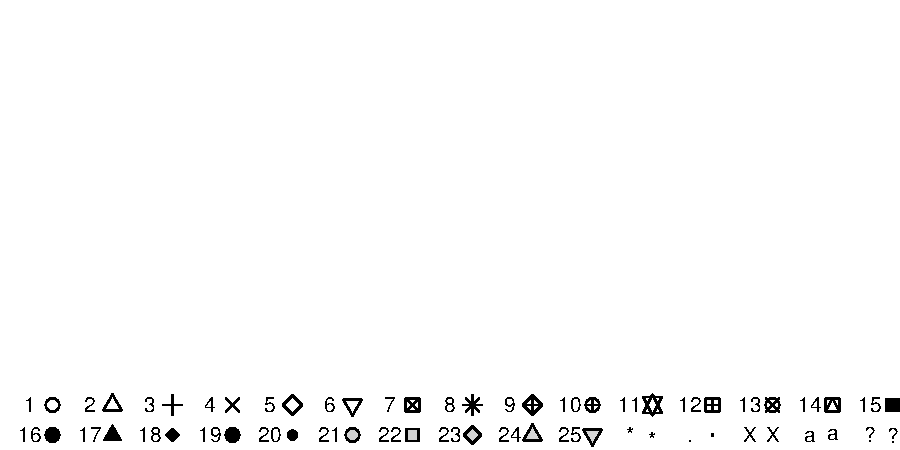
\includegraphics[width=8.5cm]{files/pch_symbol} 






\section{Lattice (Trellis) graphics}
\everypar={\hangindent=9mm}

\bcode{densityplot(\~{}x)}  density functions plot

\bcode{histogram(\~{}x)}  histogram of the frequencies of \code{x}

\bcode{qq(y\~{}x)}  quantiles to compare two distributions, \code{x} must be numeric, \code{y} may be numeric, character, or factor but must have two `levels'





\section{Optimization and model fitting}
\everypar={\hangindent=9mm}


\bcode{lm(formula)} fit linear models; \code{formula} is typically of
     the form \code{response ~ termA + termB + ...}; use \code{I(x*y)
     + I(x\^{}2)} for terms made of nonlinear components

\bcode{glm(formula,family=)} fit generalized linear models, specified by
     giving a symbolic description of the linear predictor and a
     description of the error distribution; \code{family} is a
     description of the error distribution and link function to
          be used in the model; see \code{?family}


\everypar={\hangindent=9mm}
\bcode{coef(fit)}  returns the estimated coefficients (sometimes with their standard-errors)

\bcode{residuals(fit)}  returns the residuals

\bcode{deviance(fit)}  returns the deviance




\section{Statistics}
\everypar={\hangindent=9mm}

\bcode{aov(formula)} analysis of variance model

\bcode{anova(fit,...)} analysis of variance (or deviance) tables for one or more
     fitted model objects

\bcode{density(x)} kernel density estimates of \code{x}

\bcode{binom.test()}, \bcode{pairwise.t.test()}, \bcode{power.t.test()},
\bcode{prop.test()}, \bcode{t.test()}, ... use
\code{help.search("test")} 





\section{Distributions}

\bcode{rnorm(n, mean=0, sd=1)} Gaussian (normal)  

\bcode{rexp(n, rate=1)} exponential

\bcode{rgamma(n, shape, scale=1)} gamma  

\bcode{rpois(n, lambda)} Poisson

\bcode{rweibull(n, shape, scale=1)} Weibull

\bcode{rcauchy(n, location=0, scale=1)} Cauchy  

\bcode{rbeta(n, shape1, shape2)} beta

\bcode{rt(n, df)} `Student' ($t$)  

\bcode{rf(n, df1, df2)} Fisher--Snedecor ($F$)  ($\chi^2$)  

\bcode{rchisq(n, df)} Pearson 

\bcode{rbinom(n, size, prob)} binomial  

\bcode{rgeom(n, prob)} geometric  

\bcode{rhyper(nn, m, n, k)} hypergeometric  

\bcode{rlogis(n, location=0, scale=1)} logistic  

\bcode{rlnorm(n, meanlog=0, sdlog=1)} lognormal  

\bcode{rnbinom(n, size, prob)} negative binomial  

\bcode{runif(n, min=0, max=1)} uniform  

\bcode{rwilcox(nn, m, n)}, \code{rsignrank(nn, n)} Wilcoxon's statistics  

All these functions can be used by replacing the letter \code{r} with
\code{d}, \code{p} or \code{q} to get, respectively, the probability
density (\code{d\textsl{func}(x, ...)}), the cumulative probability
density (\code{p\textsl{func}(x, ...)}), and the value of quantile
(\code{q\textsl{func}(p, ...)}, with 0 $<$ \code{p} $<$ 1).


\section{Programming}
\everypar={\hangindent=9mm}

\bcode{function( arglist ) expr} function definition

\bcode{return(value)}

\everypar={\hangindent=0mm}
\bcode{if(cond) expr\\
if(cond) cons.expr  else  alt.expr\\
for(var in seq) expr\\
while(cond) expr\\
break\\
next}

Use braces \{\} around statements


\everypar={\hangindent=9mm}
\bcode{ifelse(test, yes, no)} a value with the same shape as \code{test} filled with elements
from either \code{yes} or \code{no} 


\end{multicols*}
\end{document}
